\documentclass{beamer}
\usepackage{graphicx} % Required for inserting images
\usepackage[T1]{fontenc} % Wichtig für Trennung von Wörtern
\usepackage[utf8]{inputenc} % Erlaubt Umlaute im Code
\usepackage[ngerman]{babel}
\usepackage{bbm}
\usepackage{amsmath}
\usepackage{amssymb}
\usepackage{amsthm}
\usepackage{mathtools}
\usepackage{csquotes}
\usepackage{url}






% Package zum verweisen auf Literatur
\usepackage[style=verbose]{biblatex}
\addbibresource{Slides_Literatur.bib}

\newcommand{\N}{\mathbbm{N}} % natürliche Zahlen
\newcommand{\Z}{\mathbbm{Z}} % ganze Zahlen
\newcommand{\R}{\mathbb{R}} % reelle Zahlen
\newcommand{\C}{\mathbb{C}} % komplexe Zahlen
\newcommand{\Q}{\mathbb{Q}} % rationale Zahlen


% Einstellungen für Template
\setbeamertemplate{footline}[frame number]
\setbeamertemplate{theorems}[numbered]
\setbeamertemplate{section in toc}[sections numbered]
\setbeamertemplate{subsection in toc}[subsections numbered]
\setbeamerfont{footnote}{size=\tiny}


\newtheorem{satz}{Satz}[section]
\newtheorem{defn}[satz]{Definition}
\newtheorem{lem}[satz]{Lemma}
\newtheorem{beispiel}[satz]{Beispiel}

% Überschrift soll Gliederung folgen
\newif\ifshowtoc
\showtoctrue % Standardmäßig auf "wahr"


\AtBeginSection[]
{
  \begin{frame}{Übersicht}
    \tableofcontents[
      currentsection,
      sectionstyle=show/shaded,
      subsectionstyle=show/show/hide
    ]
  \end{frame}
}

% Automatisierung der Titel der Folien:
\newcommand{\secframe}{\begin{frame}{\insertsectionnumber. \insertsection}}
\newcommand{\subsecframe}{\begin{frame}{\insertsectionnumber.\insertsubsectionnumber \ \insertsubsection}}



\title{Proseminar: Darstellungen ganzer Zahlen}
\author{Carl-Philip Deerberg}
\date{21.04.2026}

\begin{document}

% Title Slide
\begin{frame}[plain]
    \titlepage
\end{frame}

% Inhaltsverzeichnis am Anfang

\begin{frame}{Gliederung}
    \tableofcontents[hideallsubsections]
\end{frame}


\section{Einführung}
    \subsection{Warum ganze Zahlen darstellen?}
        \subsecframe
            \begin{figure}
                \centering
                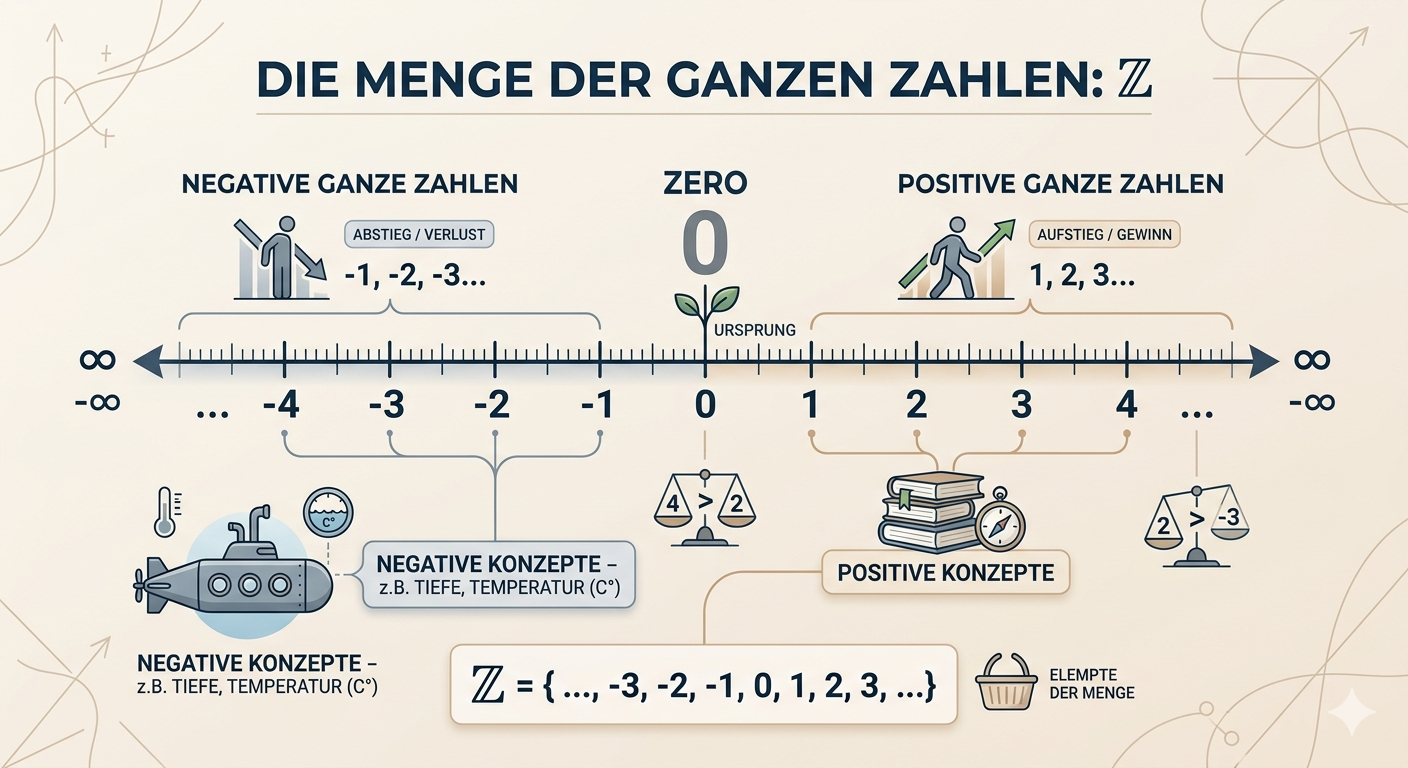
\includegraphics[width=0.99\textwidth]{ganze-zahlen.jpg} 
                \footnote{Grafik erstellt mit Gemini - Nano Banana 2}
            \end{figure}
        \end{frame}
        \subsecframe
            Ganze Zahlen sind für Menschen gut vorstellbar. \\
            Menschen können gut mit der bekannten Zahlenvorstellung arbeiten und rechnen. \\
            Speicherung und Darstellung auf Papier: Kein Problem.
        \end{frame}

    \subsection{Zahlen im Computer}
        \subsecframe
            Aber: \\
            Wie können Computer mit (ganzen) Zahlen arbeiten?
            \begin{itemize}
                \item Computer kennen keine ``Zahlen''
                \item Computer arbeiten mit Strom(-signalen)
                \item Physikalisch gesehen zwei mögliche Zustände: \\
                    Spannung an / Spannung aus
            \end{itemize}
        \end{frame}
        \subsecframe
            \begin{figure}
                \centering
                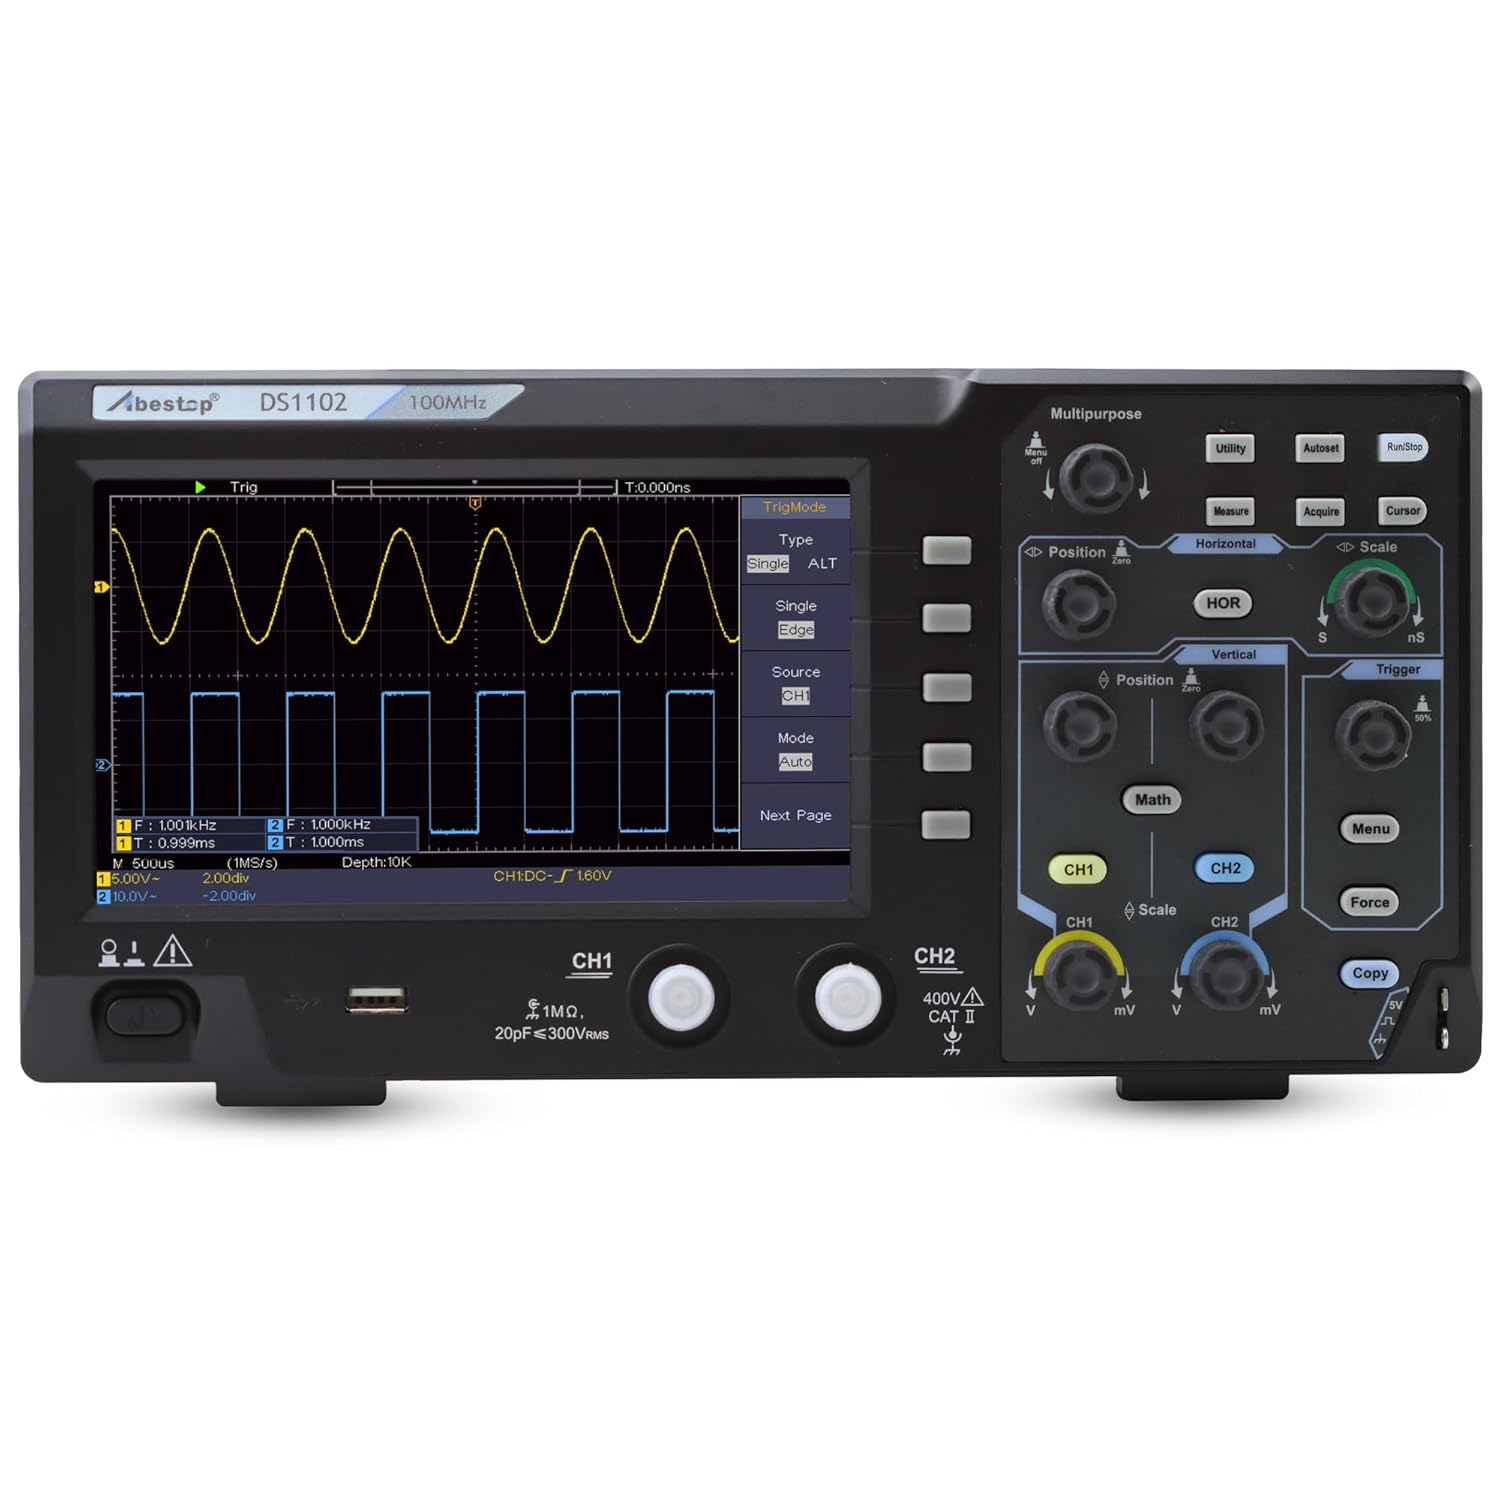
\includegraphics[width=0.8\textwidth]{oszilloskop.jpg} 
            \end{figure}
            Bits - Strom an / Strom aus
        \end{frame}

        \subsecframe
            Diese Signale lassen sich als \textbf{Bits} auffassen
            \begin{itemize}
                \item Bit: ``Binary Digit'' (Binärziffer)
                \item Kleinste Informationseinheit der Digitaltechnik
                \item Zwei Zustände: ``1'' oder ``0'' \\
                    Entsprechen ``Strom an'' oder ``Strom aus''
            \end{itemize}
        \end{frame}

        \subsecframe
            Lassen sich also nur zwei Zustände in Computern speichern? 
            \\ $\rightarrow$ Nein!
            \begin{itemize}
                \item \textit{Alle} Informationen lassen sich mit Bits kodieren
                \item Ein Bit: $2^1 = 2$ Zustände
                \item Vier Bits: $2^4 = 16$ Zustände bzw. Kombinationen
            \end{itemize}
        \end{frame}

        \subsecframe
            Also stellen wir uns die Frage: \\
            Wie können wir ganze Zahlen darstellen, damit wir sie im Computer verarbeiten können? \footcite[Der Vortrag hierzu basiert auf:][]{hougardy2018}
        \end{frame}

\section{Ganze Zahlen}


    \subsection{Mathematische Beschreibung der ganzen Zahlen}      
        \subsecframe
            Erinnerung an die Definition der natürlichen Zahlen:
            \begin{defn}[Induktive Mengen]
                Eine Menge $S \subset \R$ heißt \textbf{induktiv}, wenn sie die folgenden zwei Bedingungen erfüllt:
                \begin{itemize}
                    \item $1 \in S$.
                    \item $x \in S ~\Rightarrow~ x+1 \in S$. \\
                        $x+1$ heißt \textbf{Nachfolger} von $x$. \footcite{grigor2024}
                \end{itemize}
            \end{defn}
            \begin{defn}[Natürliche Zahlen] \label{def:nat-zahlen}
                Die Menge $\N$ der natürlichen Zahlen ist der Durchschnitt von allen induktiven Mengen.  \\
                Oder: \[\N \coloneq \{1,2,3, \dots\}\]
            \end{defn}
        \end{frame}

        \subsecframe
            \begin{block}{Definition \ref{def:nat-zahlen} (Natürliche Zahlen)}
                Die Menge $\N$ der natürlichen Zahlen ist der Durchschnitt von allen induktiven Mengen.\footcite{grigor2024}  \\
                Oder: \[\N \coloneq \{1,2,3, \dots\}\]                
            \end{block}
            \begin{block}{Anmerkung}
                Bei den im Folgenden betrachteten Darstellungsweisen von Zahlen kann auch die alternative Definition
                \[\N = \{0,1,2,3,\dots\}\]
                verwendet werden.
            \end{block}
        \end{frame}

        \subsecframe
            \begin{defn} [Ganze Zahlen]
                Die Menge $\Z$ von \textbf{ganzen Zahlen} wird wie folgt definiert:
                \[\Z \coloneq \{0\} \cup \N \cup (-\N), \]
                wobei $-\N \coloneq \{-n \colon n \in \N\}$ die Menge von den Negativen der natürlichen Zahlen ist.\footcite{grigor2024} \\
                Oder: \[\Z \coloneq \{\dots, -3,-2,-1,0,1,2,3,\dots\}\]
            \end{defn}
        \end{frame}


    \subsection{Operationen mit ganzen Zahlen}
        \subsecframe
            \begin{satz}[Operationen in $\Z$]
                Für alle $x,y\in \Z$ sind $x+y,~x-y,~xy$ auch in $\Z$.\footcite{grigor2024}
            \end{satz}
            D.h., die gewöhnlichen Rechenoperationen Addition, Subtraktion und Multiplikation lassen sich mit den ganzen Zahlen durchführen. \\
            Merke: \\
            Mit allen Darstellungsformen für ganze Zahlen müssen diese Operationen auch ausgeführt werden können.
        \end{frame}

    
%    \subsection{Induktionsprinzip}
%        \subsecframe
%            Da die natürlichen Zahlen auf diesem Prinzip aufgebaut sind und wir es in Beweisen benötigen:
%            \begin{satz}[Induktionsprinzip]
%                Sei $A(n)$ eine von $n\in \N$ abhängige Aussage, d.h \[A \colon \N \to \{\text{wahr, falsch}\}.\]
%                Nehmen wir an, dass $A$ die folgenden zwei Bedingungen erfüllt:
%                \begin{itemize}
%                    \item $A(1)$ ist wahr.
%                    \item Für jedes $n\in \N$ gilt $A(n) \Rightarrow A(n+1)$.
%                \end{itemize}
%                Dann ist $A(n)$ wahr für alle $n\in\N$.\footcite{grigor2024}
%            \end{satz}
%        \end{frame}
    


\section{b-adische Darstellung natürlicher Zahlen}

    \secframe
        Zurück zur Darstellung von Zahlen... \\
        Wir betrachten zunächst eine Möglichkeit zur Darstellung von \textbf{natürlichen Zahlen} \\
        \begin{itemize}
            \item Zahlen sind diskret unterscheidbar
            \item Kein Vorzeichen zu beachten \\
                \textit{Die Bedeutung des Vorzeichens sehen wir später...}
        \end{itemize}
    \end{frame}

    \secframe
        Eine Möglichkeit zur alternativen Darstellung von natürlichen Zahlen: \\  
        \vspace{\baselineskip}
        \begin{itemize}
            \item $b$-adische Darstellung für natürliche Zahlen
        \end{itemize}
        \vspace{\baselineskip}
        Übliche Darstellungsform für natürliche Zahlen \\
        Bekannte Variante der $b$-adischen Darstellung:
        \begin{itemize}
            \item Binärdarstellung
        \end{itemize}
    \end{frame}

    \subsection{Beispiel zur b-adischen Darstellung: Binärdarstellung}

        \subsecframe
            Beispiel zur Darstellung von natürlichen Zahlen: \textbf{Binärdarstellung} \\
            \textit{(``$2$-adische Darstellung'')}
            \begin{beispiel} \label{bsp:Binär}
                Die Zahl $106$ lässt sich zerlegen als:
                \begin{align}
                    106 &= 1 \cdot 10^2 + 0 \cdot 10^1 + 6 \cdot 10^0 \label{bsp:Binär_Dez}\\
                    &= 1 \cdot 2^6 + 1 \cdot 2^5 + 0 \cdot 2^4 + 1 \cdot 2^3 + 0 \cdot 2^2 + 1 \cdot 2^1 + 0 \cdot 2^0 \label{bsp:Binär_Bin}
                \end{align}
                Aus (\ref{bsp:Binär_Dez}) folgt die gewohnte Dezimaldarstellung: $106$. \\
                Aus (\ref{bsp:Binär_Bin}) folgt die Binärdarstellung: \[106 = 1101010\]
            \end{beispiel}
        \end{frame}

        \subsecframe
            \begin{block}{Beispiel \ref{bsp:Binär}}
                \begin{align*}
                    106 &= 1 \cdot 10^2 + 0 \cdot 10^1 + 6 \cdot 10^0 \\
                    &= 1 \cdot 2^6 + 1 \cdot 2^5 + 0 \cdot 2^4 + 1 \cdot 2^3 + 0 \cdot 2^2 + 1 \cdot 2^1 + 0 \cdot 2^0 
                \end{align*}
                Binärdarstellung:
                \[106 = 1101010\]
                \begin{itemize}
                    \item Besteht nur noch aus zwei Zuständen: ``1'' und ``0''.
                \end{itemize}
            \end{block}
            Dies nennt man die $b$-adische Darstellung zur Basis $b=2$.
        \end{frame}

        \subsecframe
            Lässt sich diese Zerlegung auf alle natürlichen Zahlen anwenden?
            \begin{itemize}
                \item Ja! 
                \item Und man kann statt $10$ oder $2$ auch jede beliebige Basis $b \in \N,~b\geq 2$ nehmen! 
            \end{itemize}
            Beides zeigt uns der folgende Satz:
        \end{frame}

    \subsection{b-adische Darstellung: Allgemeine Formulierung}

        \subsecframe
            \begin{satz}[b-adische Darstellung für natürliche Zahlen] \label{satz:b-adische_Darstellung}
                Sei $b\in \N, b \geq 2$, $n \in \N$.
                Dann existieren $l \in \N$ und $z_i \in \{0, \dots, b-1\}, {i = 0, \dots, l-1},$ eindeutig bestimmt, welche die Bedingungen $z_{l-1} \neq 0$ und 
                \begin{equation}
                    n = \sum_{i=0}^{l-1}z_ib^i \label{eq:b-adische_Darstellung_n}
                \end{equation}
                erfüllen. \\
                Das Wort $z_{l-1}\dots z_0$ heißt die \textbf{b-adische Darstellung} von n.\\
                Man schreibt auch $n=(z_{l-1} \dots z_0)_b$. \\
                Stets gilt für die Länge der Darstellung:
                    \begin{equation}
                        l-1 = \lfloor \log_b n \rfloor. \label{eq:b-adische_Darstellung_log}
                    \end{equation}
            \end{satz}
        \end{frame}

        \subsecframe
            Für den Beweis benötigen wir das folgende Lemma:
            \begin{lem} \label{lemma:Eindeutigkeit_b-adische_Darstellung}
                Sei $k \in \N$ und $l \in \N$. 
                Definiere $f^l \colon \{0, \dots, k-1\}^l \to \{0, \dots, k^l-1\}$ durch $f^l(w) \coloneq \sum_{i=1}^l a_i k^{l-i}$ für alle $w=a_1 \dots a_l \in \{0, \dots, k-1\}^l$.
                Dann ist $f^l$ wohldefiniert und bijektiv.
            \end{lem}
            \begin{proof}
                Vergleiche den Vortrag in der letzten Woche \footcite{chung2026} und \footcite[S. 17, Lemma 1.19]{hougardy2018}.
            \end{proof}
        \end{frame}

        \subsecframe
            \begin{proof}[Beweis (von Satz \ref{satz:b-adische_Darstellung})]
                Zunächst beweisen wir \ref{satz:b-adische_Darstellung} \eqref{eq:b-adische_Darstellung_log}: $l-1 = \lfloor \log_b n \rfloor$.\\
                \vspace{\baselineskip}
                Es gilt: \[n \geq z_{l-1}b^{l-1} \geq 1\cdot b^{l-1}\]
                und \[n \leq \sum_{i=0}^{l-1} (b-1)b^i = (b-1) \frac{b^l-1}{b-1} = b^l - 1 < b^l\]
                Also:
                \begin{align*}
                    &b^{l-1} \leq n < b^l \\
                    \Rightarrow &{l-1} \leq \log_b (n) < l \\
                    \Rightarrow &l-1 = \lfloor \log_b(n) \rfloor
                \end{align*}
            \end{proof}
        \end{frame}

        \subsecframe
            \begin{proof}[Beweis (von Satz \ref{satz:b-adische_Darstellung}): Eindeutigkeit]
                Beweis der Eindeutigkeit der Darstellung: \\
                \vspace{\baselineskip}
                Voraussetzung: Länge $l$ gegeben durch $l = \lfloor logb(n) \rfloor + 1$ \\
                \vspace{\baselineskip}
                Wir nutzen die Abbildung $f_l$ aus Lemma \ref{lemma:Eindeutigkeit_b-adische_Darstellung}: \\
                Da $f_l$ bijektiv und insbesondere injektiv, erzeugt genau eine Ziffernfolge $(z_i)_{i=0,\dots,l-1}$ den Wert $n$. \\
                
            \end{proof}
        \end{frame}

        \subsecframe
            \begin{block}{Beweis (von Satz \ref{satz:b-adische_Darstellung}): Existenz}
                Beweis der Existenz durch vollständige Induktion über $l(n) = 1 + \lfloor \log_b(n) \rfloor$. \\
                \vspace{\baselineskip}
                Induktionsanfang: $l(n) = 1$.
                \begin{itemize}
                    \item $\Rightarrow \lfloor \log_b(n) = 0 \rfloor$
                    \item Gilt für $b^0 \leq n < b^1$
                    \item Also $1 \leq n < b$
                    \item Darstellung $n = z_0 b^0 = z_0$ ist trivial, da $n$ selbst
                \end{itemize}
            \end{block}
        \end{frame}

        \subsecframe
            \begin{proof}[Beweis (von Satz \ref{satz:b-adische_Darstellung}): Existenz]
                \textbf{Induktionsschritt:} $l-1 \to l$. Sei $l \geq 2$. \\
                Wir setzen $n' = \lfloor \frac{n}{b} \rfloor.$
                Die Länge von $n'$ ist $l' = l-1$. \\
                \vspace{\baselineskip}
                \textbf{Induktionsvoraussetzung:} Für $n'$ ex. Darstellung $\displaystyle\sum_{i=0}^{l'-1} z'_i b^i.$ \\
                Division mit Rest ergibt: $n = n' \cdot b + z_0$ mit $z_0 = n \bmod b$. \\
                \[\Rightarrow n = b \cdot \left( \sum_{i=0}^{l'-1} z'_i b^i \right) + z_0 = \sum_{i=0}^{l'-1} z'_i b^{i+1} + z_0\] 
                Mit $j= i+1$ und $z_j = z'_{j-1}$ folgt $n = \displaystyle\sum_{j=0}^{l-1}z_jb^j.$
            \end{proof}
        \end{frame}

        \subsecframe
            Anmerkung: \\
            Die Rechenoperationen innerhalb der natürlichen Zahlen funktionieren mit der $b$-adischen Darstellung analog.
            \begin{itemize}
                \item Ähnlich wie beim schriflichen Rechnen mit Übertrag
            \end{itemize}
        \end{frame}

    \subsection{b-adische Darstellung: Anwendung des Satzes}        

        \subsecframe
            \begin{beispiel}\label{bsp:b-adisch}
                Wir wollen die Zahl $n=13$ in Binärdarstellung darstellen, also zur Basis $b=2$.
            \end{beispiel}
            \vspace{\baselineskip}
            \textbf{Schritt 1:} Länge $l$ berechnen. 
            Es gilt: $l-1 = \lfloor \log_b(n) \rfloor$. \\
                \[8 \leq 13 < 16 \Leftrightarrow 2^3 \leq 13 < 2^4\]
            $\log$ anwenden:
                \[\log_2(2^3) \leq \log_2(13) < \log_2(2^4) \Leftrightarrow 3 \leq \log_2(13) < 4\]
            Also: $\lfloor \log_2(13) \rfloor = 3$ und es folgt
            \[l-1 = 3 \Leftrightarrow l = 3+1=4\]
        \end{frame}        

        \subsecframe
            \begin{block}{Beispiel \ref{bsp:b-adisch}}
                Wir wollen die Zahl $n=13$ in Binärdarstellung darstellen, also zur Basis $b=2$.
            \end{block}        
            \vspace{\baselineskip}
            \textbf{Schritt 2:} Wir bestimmen $z_0, \dots, z_3$.
            \begin{align*}
                &z_0\colon 13 : 2 = 6  \text{ Rest }1 \Rightarrow z_0 = 1 \\
                &z_1\colon 6 : 2 = 3  \text{ Rest }0 \Rightarrow z_1 = 0 \\
                &z_2\colon 3 : 2 = 1  \text{ Rest }1 \Rightarrow z_2 = 1 \\
                &z_3\colon 1 : 2 = 0  \text{ Rest }1 \Rightarrow z_3 = 1 \\
            \end{align*}
            \vspace{\baselineskip}
            \textbf{Schritt 3:} Einsetzen in b-adische Formel:
            \[13 = 1 \cdot 2^3 + 1\cdot 2^2 + 0 \cdot 2^1 + 1 \cdot 2^0\]
            Also ist die Binärdarstellung von $13 = (1101)_2$
        \end{frame}        

    \secframe
        Was haben wir gesehen?
        \begin{itemize}
            \item Natürliche Zahlen können in $b$-adischer Form als Wörter dargestellt werden
            \item Häufige Darstellungsform: Binärdarstellung
            \item Umrechnung von klassischer zu Binärdarstellung
        \end{itemize}
    \end{frame}

    

\section{b-Komplementdarstellung ganzer Zahlen}

    \secframe
        Stellt sich jetzt die Frage:
        \begin{itemize}
            \item Wir können wir ganze Zahlen so darstellen, dass diese ebenfalls für Computer verarbeitbar sind?
        \end{itemize}
    \end{frame}

    \subsection{Natürliche Zahlen und Ganze Zahlen - Unterschied}

        \subsecframe
            Unterschied bei der gewöhnlichen Darstellung:
            \begin{itemize}
                \item Wir setzen ein negatives Vorzeichen $(-)$ vor ein Element der natürlichen Zahlen
            \end{itemize}
            Idee:
            \begin{itemize}
                \item Wir ``kodieren'' das erste der dargestellten Bits als Vorzeichen!
                \item Man spricht von einer ``Vorzeichen-'' oder ``Betragsdarstellung''
            \end{itemize}
        \end{frame}

        \subsecframe
            \begin{beispiel}{Betragsdarstellung von ganzen Zahlen} \label{bsp:Betragsdarstellung}
                Binärdarstellung mit 4 Bits, wobei das erste das Vorzeichen darstellt. \\
                $0$ entspricht $(+)$, $1$ entspricht $(-)$. \\
                Dann lassen sich die Zahlen $-7$ bis $+7$ darstellen als:
                \begin{align*}
                0 \Leftrightarrow 0000  ~&;~  -0 \Leftrightarrow 1000 \\
                1 \Leftrightarrow 0001  ~&;~  -1 \Leftrightarrow 1001 \\
                & \vdots \\
                7 \Leftrightarrow 0111  ~&;~  -7 \Leftrightarrow 1111
                \end{align*}
            \end{beispiel}
        \end{frame}

        \subsecframe
            Schwierigkeiten dieser Darstellung:
            \begin{itemize}
                \item Mehrere verschiedene Darstellungen für die gleiche Zahl: \\
                    $0 \Leftrightarrow 0000$ und $0 \Leftrightarrow 1000$
                \item Rechenoperationen funktionieren nicht wie gedacht: \\
                    Da $2 + (-1) = 1$, muss gelten $0010 + 1001 = 0001$ \\
                    $\Rightarrow$ Keine spaltenweise (=bitweise) Addition möglich
            \end{itemize}
            \vspace{\baselineskip}
            Also: Andere Darstellungsform notwendig.
        \end{frame}

    \subsection{b-Komplementdarstellung: Beispiel}

        \subsecframe
            Wir identifizieren jede negative Zahl $z \in \{-2^{l-1}, \dots, -1\}$ mit $z + 2^l$. \\
            $l$ sei hier wie bisher die Länge der Zahl, also die Anzahl der verwendeten Bits.
        \end{frame}

        \subsecframe
            \begin{beispiel}
                Darstellung von $z=-3$ als $b$-Komplement mit $l=4$ Bits:
                \[z + 2l = -3 + 16 = 13\]
                $13$ wird in Binärform zu $1101$. Die Bits werden interpretiert als:
                \begin{align*}
                    &\text{Bit 3: } -2^3 = -8 \\
                    &\text{Bit 2: } 2^2 = 4 \\
                    &\text{Bit 1: } 2^1 = 2 \\
                    &\text{Bit 0: } 2^0 = 1
                \end{align*}                
                Konkret für $1101$:
                \[(1 \cdot (-8)) + (1 \cdot 4) + (0 \cdot 2) + (1 \cdot 2) = -3\]
            \end{beispiel}
        \end{frame}

        \subsecframe
            Mit 4 Bits lassen sich also die folgenden Zahlen darstellen:
            \begin{align*}
                0 \Leftrightarrow 0000  ~&;~  -8 \Leftrightarrow 1000 \\
                1 \Leftrightarrow 0001  ~&;~  -7 \Leftrightarrow 1001 \\
                & \vdots \\
                7 \Leftrightarrow 0111  ~&;~  -1 \Leftrightarrow 1111
            \end{align*}    
            Die Addition funktioniert hier auch wie bereits beschrieben:
            \begin{align*}
                &0010 \text{ (also } 2) \\
                +~ &1001 \text{ (also } -7) \\
                =~ &1011 \text{ (also } -5)
            \end{align*}
        \end{frame}

    \subsection{b-Komplementdarstellung: Allgemeine Formulierung}

        \subsecframe
            \begin{defn}[$b$-Komplement] \label{def:b-Komplement}
                Seien $l,b \in \N$, mit $b\geq 2$, sei $n \in \{0, \dots, b^l-1\}$. \\
                \vspace{\baselineskip}
                Dann ist 
                \[K^l_b(n) \coloneq (b^l-n) \bmod b^l\]
                das $l$-stellige $b$-Komplement von $n$. \\
                \vspace{\baselineskip}
                Für die Basis $b=2$ nennt man $K_2$ das Zweierkomplement, für $b=10$ nennt man $K_{10}$ das Zehnerkomplement.
            \end{defn}
        \end{frame}

        \subsecframe
            \begin{lem}[$b$-Komplement einer Zahl berechnen]\label{lem:b-Komplement_berechnen}
                Seien $l,b \in \N$, mit $b\geq 2$. Sei $n=\sum_{i=0}^{l-1} z_ib^i$ mit $z_i \in \{0, \dots, b-1\}$ für $i = 0, \dots, l-1$.
                Dann gilt:
                \begin{enumerate}[(i)]
                \item $K^l_b(n+1) = \displaystyle\sum_{i=0}^{l-1}(b-1-z_i)b^i, \text{ falls } n\neq b^l-1$ \label{lem:b-Komplement_berechnen_Berechnung}
                \item $K^l_b(0)=0$ \label{lem:b-Komplement_berechnen_von0} 
                \item $K^l_b(K^l_b(n))=n$ \label{lem:b-Komplement_berechnen_KomplementKomplement} 
                \end{enumerate}                
            \end{lem}
        \end{frame}

        \subsecframe
            \begin{proof}[Beweis von Lemma \ref{lem:b-Komplement_berechnen} (\ref{lem:b-Komplement_berechnen_von0})]
                Folgt aus Definition des $b$-Komplements (\textit{Definition \ref{def:b-Komplement}}):
                \[K_l^b(n) = (b^l-n) \bmod b^l\]
                mit $n=0$:
                \[K_l^b(0)=(b^l-0) \bmod b^l = b^l \bmod b^l = 0\]
            \end{proof}
        \end{frame}

        \subsecframe
            \begin{proof}[Beweis von Lemma \ref{lem:b-Komplement_berechnen} (\ref{lem:b-Komplement_berechnen_Berechnung})]
                Sei $n \neq b^l-1$, also $n\in \{0, \dots, b^l -2\}$. \\
                Nach Definition: $K_l^b(m) = (b^l - m) \bmod b^l$ \\
                \vspace{\baselineskip}
                Für $m = n + 1$ gilt: $1 \le m \le b^l - 1$. \\
                Daraus folgt: $K_l^b(n+1) = b^l - (n+1) = b^l - 1 - n$ \\
                \vspace{\baselineskip}
                Es gilt die geometrische Reihe: $b^l - 1 = \displaystyle\sum_{i=0}^{l-1} (b - 1)b^i$ \\
                \vspace{\baselineskip}
                Einsetzen von $n$ ergibt: $K_l^b(n+1) = \displaystyle\sum_{i=0}^{l-1} (b - 1 - z_i)b^i$
            \end{proof}
        \end{frame}

        \subsecframe
            \begin{proof}[Beweis von Lemma \ref{lem:b-Komplement_berechnen} (\ref{lem:b-Komplement_berechnen_KomplementKomplement})]
                zz.: $K_l^b(K_l^b(n)) = n$ \\
                \vspace{\baselineskip}
                Für $n=0$ gilt nach (\ref{lem:b-Komplement_berechnen_von0}): 
                \[K^b_l(K^b_l(0)) = K^b_l(0) = 0\]
                Für $n \in \{1, \dots, b1{l-1}\}$, setzen wir $m \coloneq K_l^b(n) = b^l -n$. \\
                Dann gilt:
                \[K_l^b(m) = (b^l - m) \bmod b^l = (b^l - (b^l - n)) \bmod b^l = n \bmod b^l\]
                Da $n < b^l$, gilt $n \bmod b^l = n$. \\
                $\Rightarrow K_l^b(K_l^b(n)) = n$
            \end{proof}
        \end{frame}

    \subsection{b-Komplementdarstellung: Beispiel zum Lemma}

        \subsecframe
            \begin{beispiel}[$b$-Komplement berechnen mit Lemma \ref{lem:b-Komplement_berechnen} (\ref{lem:b-Komplement_berechnen_Berechnung})]
                Sei $b=10$, $l=4$. Wir berechnen $K_4^{10}(4809)$. \\
                \begin{itemize}
                    \item $n+1 = 4809 \Rightarrow n = 4808$
                    \item $n=4 \cdot 10^3 + 8 \cdot 10^2 + 0\cdot 10^1 + 8\cdot 10^0$ \\
                        $\Rightarrow z_3 = 4, z_2 = 8, z_1 = 0, z_0 =8$
                    \item   \begin{align*}
                                K_4^{10}(4808+1) &= \sum_{i=0}^3(10-1-z_i)10^i \\
                                &= (9-4) \cdot 10^3 + (9-8) \cdot 10^2 \\ 
                                &~~+ (9-0) \cdot 10^1 + (9-8) \cdot 10^0 \\
                                &= 5 \cdot 10^3 + 1 \cdot 10^2 + 9 \cdot 10^1 + 1 \cdot 10^0
                            \end{align*}
                \end{itemize}
                Also ist $K_4^{10}(4809) = (5191)_{10}$.
            \end{beispiel}
        \end{frame}

        \subsecframe
            \begin{beispiel}[$b$-Komplement berechnen mit Lemma \ref{lem:b-Komplement_berechnen} (\ref{lem:b-Komplement_berechnen_Berechnung})]
                Sei $b=2$, $l=4$. Wir berechnen $K_4^2(6)$, $6 = (0110)_2$.\\
                \begin{itemize}
                    \item $n+1 = (0110)_2 \Rightarrow n = (0110)_2 -1 = (0101)_2$
                    \item $n=0 \cdot 2^3 + 1 \cdot 2^2 + 0\cdot 2^1 + 1\cdot 2^0$ \\
                        $\Rightarrow z_3 = 0, z_2 = 1, z_1 = 0, z_0 =1$
                    \item   \begin{align*}
                                K_4^2((0110)_2) &= \sum_{i=0}^3(2-1-z_i)2^i = \sum_{i=0}^3(1-z_i)2^i \\
                                &= (1-0) \cdot 2^3 + (1-1) \cdot 2^2 + (1-0) \cdot 2^1 + (1-1) \cdot 2^0 \\
                                &= 1 \cdot 2^3 + 0 \cdot 2^2 + 1\cdot 2^1 + 0\cdot 2^0 \\
                                &= (1010)_2
                            \end{align*}
                \end{itemize}
                Also ist $K_4^2((0110)_2) = (1010)_2$.
            \end{beispiel}
        \end{frame}

    \secframe
        Was haben wir gesehen?
        \begin{itemize}
            \item Ganze Zahlen als $b$-Komplement darstellen
            \item Übergang von klassischer Darstellung zu $b$-Komplementdarstellung
        \end{itemize}
        \vspace{\baselineskip}
        Ein Problem für die Verarbeitung im Computer bleibt bei der $b$-Komplementdarstellung: \\
        Die Zahlen sind je nach Größe unterschiedlich ``lang''.
        \begin{itemize}
            \item Problem für die Durchführung von Rechenoperationen
        \end{itemize}
        Ausweg:
        \begin{itemize}
            \item $l$-stellige $b$-Komplementdarstellung von ganzen Zahlen
        \end{itemize}
    \end{frame}


\section{l-stellige b-Komplementdarstellung ganzer Zahlen}

    \subsection{l-stellige b-Komplementdarstellung: Hintergrund}

        \subsecframe
            Eine Zahl wird nicht wie bisher in so viele Stellen bzw. Bits umgewandelt wie benötigt, sondern auf eine vorher festgelegte Länge $l$ gebracht. \\
            \vspace{\baselineskip}
            Vorteil davon:
            \begin{itemize}
                \item Computer können in festgelegtem Speicherbereich arbeiten
                \item Die Zahlen ``verlassen'' bei Rechernoperationen den festgelegten Bereich nicht
            \end{itemize}
        \end{frame}

    \subsection{l-stellige b-Komplementdarstellung: Allg. Formulierung}

        \subsecframe
            \begin{defn}[$l$-stellige $b$-Komplementdarstellung von ganzen Zahlen]
                Seien $b,l \in \N$ mit $b \geq 2$ und sei $n \in \left\{- \left\lfloor \displaystyle\frac{b^l}{2} \right\rfloor, \dots, \left\lceil \displaystyle\frac{b^l}{2} \right\rceil -1 \right\} .$
                Man erhält die $l$-stellige $b$-Komplementdarstellung von $n$, indem man die \hyperref[satz:b-adische_Darstellung]{$b$-adische Darstellung} von $n$, falls $n \geq 0$,
                bzw. die $b$-adische Darstellung von $K_b^l(-n)$, falls $n < 0$, von der vordersten Stelle mit so vielen Nullen auffüllt, bis sich eine $l$-stellige Zahl ergibt.
            \end{defn}
        \end{frame}

        \subsecframe
            \begin{itemize}
                \item Mit dieser Form kann der Computer ohne Fallunterscheidungen rechnen
                \item Einfach gesagt: \\
                    Wir können Addition und Subtraktion so durchführen, als wenn wir ausschließlich natürliche Zahlen hätten.
            \end{itemize}
            Mathematisch begründet wird das durch den folgenden Satz:
        \end{frame}

        \subsecframe
            \begin{satz}\label{satz:Rechnen_b-Komplementdarstellung}
                Seien $b,l \in \N$ mit $b \geq 2$. Setze $Z \coloneq \left\{ - \left\lfloor \displaystyle\frac{b^l}{2} \right\rfloor , \dots, \left\lceil \displaystyle\frac{b^l}{2} \right\rceil -1 \right\}$.
                Definiere die Funktion $f \colon Z \to \{0, \dots, b^l-1\}, z \mapsto 
                \begin{cases}
                    z &\text{falls } z \geq 0 \\
                    K_l^b(-z) &\text{falls } z <0
                \end{cases}$. \\
                Dann ist $f$ bijektiv und es gilt für $x,y\in Z$:
                \begin{enumerate}[i)] 
                \item Ist $x+y \in Z$, so gilt 
                    \[f(x+y) = (f(x) + f(y) \bmod b^l).\] \label{satz:Rechnen-Komplementdarstellung_Addition}
                \item Ist $x \cdot y \in Z$, so gilt 
                    \[f(x \cdot y) = (f(x) \cdot f(y)) \bmod b^l.\] \label{satz:Rechnen-Komplementdarstellung_Multiplikation}
                \end{enumerate}
            \end{satz}
        \end{frame}

        \subsecframe
            \begin{proof}[Beweis von Satz \ref{satz:Rechnen_b-Komplementdarstellung}]
                Siehe Ausarbeitung.\footcite{deerberg2026}
            \end{proof}
        \end{frame}

\section{Abschluss}

    \secframe
        Was haben wir in diesem Vortrag gesehen?
        \begin{itemize}
            \item Darstellung von natürlichen Zahlen als $b$-adisch
            \item Darstellung von ganzen Zahlen als ($l$-stelliges) $b$-Komplement
            \item Umrechnung zwischen verschiedenen Darstellungsformen
            \item Jeweils mathematische Begründungen für die Darstellungen
        \end{itemize}
    \end{frame}

    \secframe
        Vielen Dank für Eure Aufmerksamkeit!
    \end{frame}


\section*{Literatur}
\begin{frame}[allowframebreaks]{Literaturverzeichnis}
    \printbibliography
\end{frame}


\end{document}